
\chapter{*面向大语言模型智能体的机制可解释性}\label{chap:mi}

\begin{learningbox}
本章你将学习如何借助可解释人工智能与机制可解释性的工具，窥视大语言模型的黑箱内部。具体而言，你将能够：
\begin{itemize}[leftmargin=*, nosep]
    \item 区分四大可解释性范式：\textit{行为式}、\textit{归因式}、\textit{基于概念的}与\textit{机制可解释性}。
    \item 解释幻觉与{\em 忠实性}的关联，并说明机制方法如何识别导致模型失效的内部回路。
    \item 描述 Transformer 的{\em 残差流}表述，并解释信息如何跨层被迭代地精化。
    \item 应用{\em logit 透镜}与调优透镜，可视化模型预测如何逐层演化。
    \item 解释{\em 多义性与叠加}，并理解为何单个神经元是糟糕的解释单元。
    \item 使用{\em 稀疏自编码器}做字典学习，把模型激活分解为单义、人类可解释的特征。
    \item 执行{\em 回路分析与激活修补}，以识别并因果性地验证负责特定模型行为的内部算法。
\end{itemize}
\end{learningbox}

\section{打开大语言模型}
大语言模型内部是如何运作的？打开大型神经架构的黑箱，是一个重要的研究课题。我们希望理解数十亿神经元如何嵌入表征、如何推理、如何得出结论。可解释人工智能（XAI）领域提供了许多不同的方法 \citep{minh2022explainable,rios2020feature,van2022comparison,selvaraju2017grad,ali2022xai}。

来自经典机器学习社区的静态 XAI 方法一直相当成功 \citep{molnar2020interpretable}。已有方法可以把输入图片如何映射到输出类别关联起来，例如使用特征图 \citep{ren2016object,kohonen1982self,redmon2016you}。反事实分析 \citep{karimi2020model,explains24}、LIME \citep{ribeiro2016should} 与 SHAP \citep{lundberg2017unified} 等，有助于理解结构化数据中输入如何映射到输出。这些方法属于可解释性算法中的\emph{行为式}与\emph{归因式}类别，其中模型被视为黑箱（图~\ref{fig:MIconcepts}）。SHAP、LIME 等归因方法近似估计不同输入特征对最终输出的贡献。借助反事实方法实现的行为分析，则让我们了解哪些特征重要（但并不必然说明它们有多重要）。%Distillation methods can map neural networks to decision trees \citep{hinton2015distilling}, a highly interpretable machine learning method. 

\begin{figure}[!ht]
  \begin{center}
    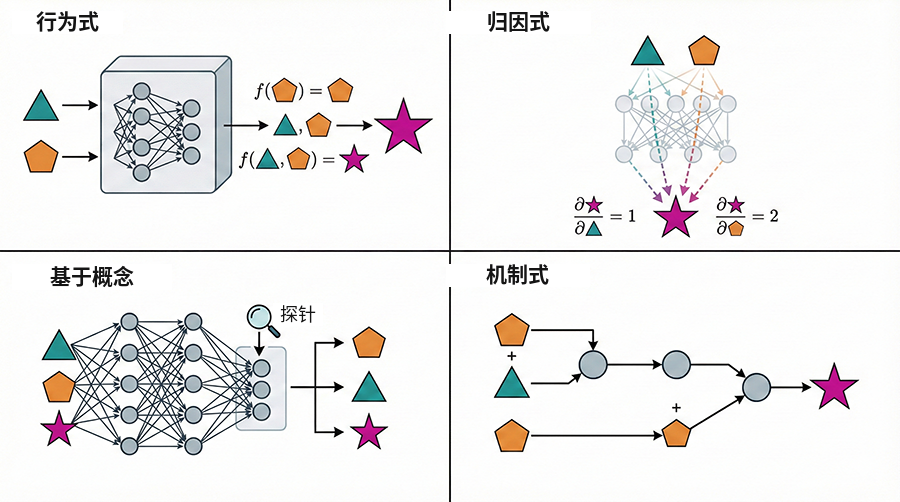
\includegraphics[width=0.9\textwidth]{figures/MI-concepts.png}
    \caption{\emph{可解释性范式}的分类。行为式可解释性把模型视为黑箱，映射输入—输出关系（$f(x) = y$）。归因式方法用梯度或显著性量化特定输入特征对最终输出的影响。基于概念的可解释性用探针识别隐藏层中高层次的、人类可理解的表征。机制可解释性旨在逆向工程出支配模型行为的具体因果回路与内部算法。\label{fig:MIconcepts}}
  \end{center}
\end{figure}

超越表层的输入—输出相关性，\emph{基于概念的}可解释性试图识别模型中是否编码了特定的、人类可理解的信息。这主要通过\emph{线性探针}来研究：在冻结的隐藏激活上训练一个简单的监督分类器，以检测特定语义概念（如词性、情感或事实实体）是否存在 \citep{alain2016understanding, belinkov2022probing}。归因方法强调输入的\textit{哪些}部分有影响，而探针则让研究者验证模型在不同层表征了\textit{什么}知识（图~\ref{fig:MIconcepts}）。然而，探针有一个已知的局限，即{\em 因果缺口}：发现某个概念在某一层被表征，并不必然意味着模型把这一信息用于最终预测。

更晚近地，人们发展出动态方法，以揭示大型 Transformer 模型内部的模式。这些方法属于机制可解释性（MI）这一子领域。MI 的目标是揭示模型动态得出结论的机制 \citep{nanda2023progress,bereska2024mechanistic,ferrando2024primer,rai2024practical}。
换言之，MI 寻求以模型的内部激活与连接来对行为给出低层次的、因果性的解释，类似于把程序的二进制反编译成可读代码。
稀疏自编码器 \citep{cunningham2023sparse,makelov2024towards}、神经透镜 \citep{black2022interpreting} 与回路发现 \citep{conmy2023towards} 等方法正被用于成功增进我们对大语言模型如何运作的洞见，例如在国际象棋中 \citep{davis2024decoding}。

XAI，尤其是 MI，是活跃的研究领域，将使我们更好地理解大语言模型如何推理、如何得出结论 \citep{sharkey2025open}。一旦获得更好的理解，大语言模型便可相应改进，例如减少幻觉。

本章将深入探讨 MI 的诸多方面。

\section{模型推理中的幻觉与忠实性}

大语言模型在高风险环境中部署的一个重大障碍是\emph{幻觉}现象：生成句法上看似合理、但事实上不正确的内容。从可解释性角度看，挑战在于区分模型的输出究竟是稳健的\emph{内部计算}的结果，还是\emph{事后辩护}。这一区分被形式化为对\emph{忠实性}的研究，即模型所陈述的推理（例如在思维链提示中）对其最终输出具有因果责任的程度。

机制可解释性（MI）提供了必要的工具，使我们超越行为层面的准确率指标，走向对模型失效模式的因果理解。例如，使用稀疏自编码器（SAE）的研究已识别出特定的\emph{诚实}回路或\emph{知识检索}回路 \citep{lindsey2025biology}。在这些研究中，研究者识别出当模型遇到不熟悉的实体时会被激活的潜在特征；当这些回路的抑制逻辑失效——即相关\emph{知识}特征激活度很低，模型却仍继续生成 token——就径直导致编造的答案。

此外，MI 让我们能够考察中间推理步骤的\emph{因果必要性}。模型可能产出一条令人信服的思维链（CoT），但它也可能已经通过另一条内部捷径算出了最终答案，只是在作为一只\emph{随机鹦鹉}生成 CoT。

为检验这一点，\citet{chen2025does} 结合\emph{因果中介分析}与 SAE，在算术任务中对潜在思维过程做干预。他们把一次启用 CoT 的运行中的潜在激活注入一次标准的零样本运行，结果表明在足够大的模型中，这些中间思维显著提升了解题置信度。这提供了经验证据：对较大的架构而言，CoT 并非仅是装饰，而是模型推理链中一条\emph{忠实}的因果链接。

反过来，较小模型中这类因果链接的缺失表明，\emph{忠实推理}可能是规模的一种涌现属性，只有当模型拥有足够参数来表征复杂多步算法时才会出现。开发量化这种忠实性的稳健指标，是人工智能安全的一个关键前沿；通过窥视模型的激活，我们有可能开发出幻觉检测器——当模型的内部置信特征与其外部言辞不一致时即触发。
\section{残差流与迭代精化} \label{residualstream}

在探讨具体的 MI 方法之前，有必要为 Transformer 架构建立一个形式化的心智模型。与经典前馈网络（每一层替换上一层的表征）不同，现代 Transformer 运行在一条\textit{残差流}上 \citep{elhage2021mathematical}。

形式上，设 $h_\ell \in \mathbb{R}^{d_{model}}$ 为第 $\ell$ 层之后的隐藏表征状态。Transformer 架构由如下递推定义：
\begin{equation}
    h_\ell = h_{\ell-1} + \mathcal{F}_\ell(h_{\ell-1})
\end{equation}
其中 $\mathcal{F}_\ell$ 表示第 $\ell$ 层所做的计算（包含多头注意力与前馈块）。


这一结构意味着最终表征 $h_L$ 是初始嵌入 $x_{embed}$ 与后续各层贡献（$\Delta h$）的累积和：
\begin{equation}
    h_L = x_{embed} + \sum_{\ell=1}^{L} \Delta h_\ell
\end{equation}

在这一视角下，残差流充当一条高维的\emph{通信通道}。各层并不变换整个状态；它们从流中读取信息、做局部计算，再通过向量加法把结果写回流中。这种可加性保证了信息能跨越许多层持续存在，更重要的是，它为模型最终输出的线性分解提供了依据。


\section{多义性与叠加}

\begin{figure}[!ht]
  \begin{center}
    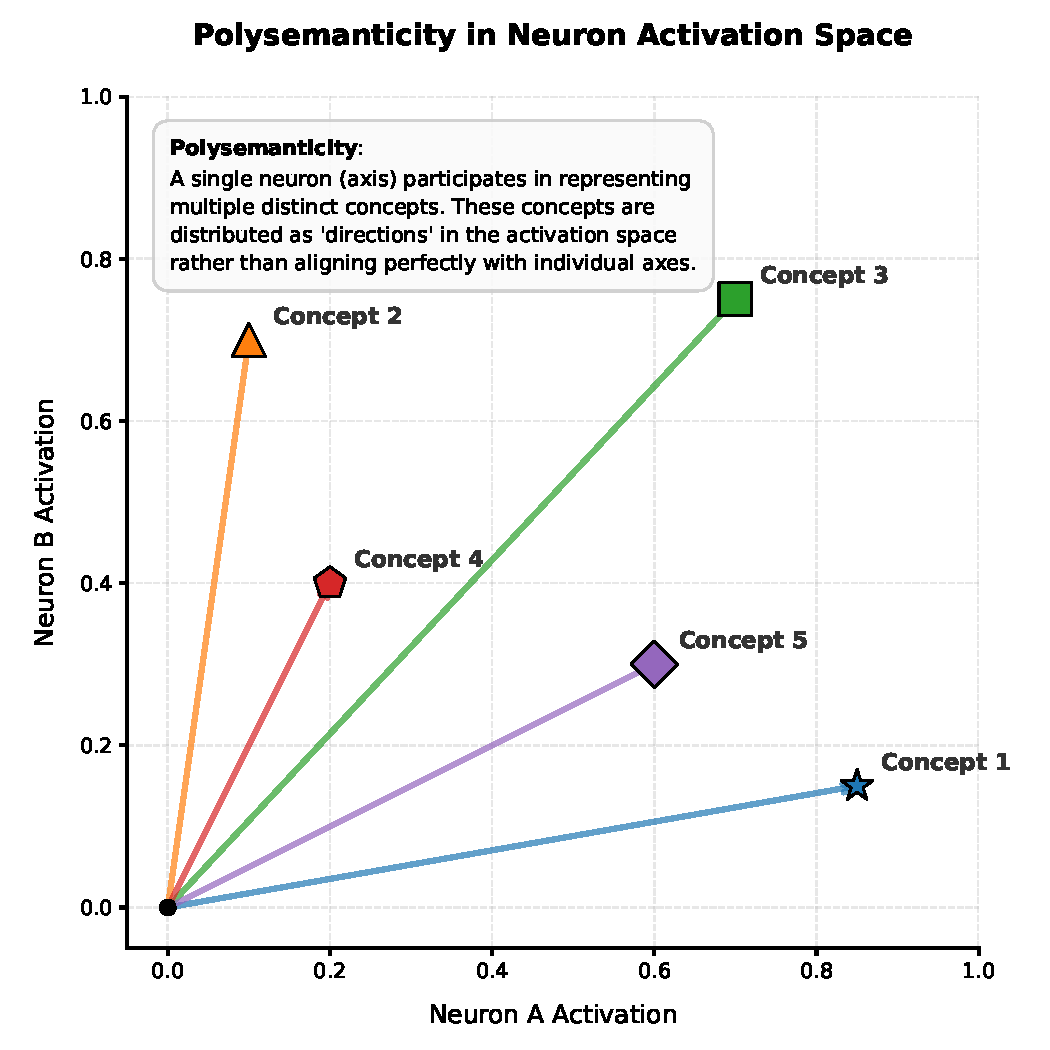
\includegraphics[width=0.9\textwidth]{figures/polysemanticity_concept_plot.pdf}
    \caption{大语言模型及其他基于 Transformer 的模型中的多义性概念 \label{fig:polysemanticity}}
  \end{center}
\end{figure}

逆向工程神经网络的一个主要瓶颈是\emph{多义性}（图~\ref{fig:polysemanticity}）：经验观察表明，单个神经元常常对多个语义上无关的概念都有激活。这一现象与\emph{叠加}密切相关——即模型用 $m$ 个维度表征 $n$ 个特征、且 $n > m$ 的情形。在\emph{线性表征假设}下，模型利用激活空间的高维几何，把特征存为近乎正交的向量。这虽带来高效的信息压缩，却造成基不匹配：固定的神经元基与真实的特征基并不对齐。

\citet{elhage2022toy} 给出了一个形式化，并用玩具模型证明：当特征稀疏时，叠加是模型最大化信息密度的一种有数学依据的策略。他们识别出特征编码中的\emph{相变}：随着某个概念的稀疏度提高，模型能在相同维度数中塞入更多特征，代价是特征之间的干扰或噪声。

为解开这种纠缠，研究者转向\emph{字典学习}，其中最著名的是\emph{稀疏自编码器}（SAE）。其目标是学到一个线性变换，把纠缠的神经元激活映射到一个维度高得多的稀疏潜空间。\citet{bricken2023monosemanticity} 成功地把这一方法用于小规模 Transformer，证明所得的 SAE 特征比原始神经元显著更具单义性、更可被人解释。这表明模型并非天生不可解释，而是我们一直用错误的坐标系在看它们。

后续工作探究了架构改动能否缓解多义性的出现。例如 \citet{liu2023seeing} 等人考察了不同激活函数或正则惩罚（如 $L_1$ 稀疏性）如何能迫使模型采用一种更对齐、更可解释的内部基。尽管有这些进展，多义性在最先进的模型中仍是普遍挑战。MI 当前的共识是：解释一个模型，需要超越「神经元即单元」的范式，转而识别模型因果逻辑实际所在的那个底层\emph{稀疏特征基}。




\section{logit 透镜}

机制可解释性中一个基本直觉是：Transformer 模型并不是在最后一层一跃算出输出，而是在\emph{残差流}中迭代地精化一个表征。\textit{logit 透镜}\footnote{最初发表于以下博文：\url{https://www.lesswrong.com/posts/AcKRB8wDpdaN6v6ru/interpreting-gpt-the-logit-lens}。更新后的实现由 \citep{wang2025logitlens4llmsextendinglogitlens} 提供。}把中间层的隐藏状态直接解码到输出词表空间，从而为这一过程提供一个窗口。

\subsection{形式机制}
考虑一个 $L$ 层的 Transformer。设 $x_0$ 为某 token 的初始嵌入，$h_\ell$ 为第 $\ell \in \{1, \dots, L\}$ 层之后的残差流状态。在标准前向传播中，最终隐藏状态 $h_L$ 经层归一化（LN）与反嵌入矩阵 $W_U \in \mathbb{R}^{d_{model} \times |V|}$ 转换为 logits $y$：
\begin{equation}
    y = \text{Softmax}(\text{LN}(h_L) W_U)
\end{equation}
logit 透镜对此加以推广：把\emph{同一个}反嵌入变换施加于中间状态 $h_\ell$：
\begin{equation}
    \hat{y}_\ell = \text{Softmax}(\text{LN}(h_\ell) W_U)
\end{equation}
其中 $\hat{y}_\ell$ 表示模型在第 $\ell$ 层的暂定概率分布。通过可视化所有层上的这些分布，研究者可以观察到\emph{信念的演化}：模型如何从模糊的语义簇走向具体的 token 预测。
\begin{figure}[!ht]
    \centering
    \resizebox{0.65\textwidth}{!}{
        \begin{tikzpicture}[
    node distance=1.2cm and 2cm,
    layer/.style={rectangle, draw, fill=gray!10, minimum width=3cm, minimum height=0.8cm, font=\small\sffamily, rounded corners=2pt},
    stream/.style={-{Stealth}, line width=1.5pt, color=gray!60},
    lens_path/.style={-{Stealth}, line width=1.2pt, color=teal, dashed},
    box/.style={rectangle, draw, fill=white, font=\scriptsize\sffamily, inner sep=4pt, rounded corners=1pt},
    lens_box/.style={rectangle, draw=teal!70!purple, fill=teal!5, thick, font=\scriptsize\sffamily, inner sep=5pt, rounded corners=1pt, align=center},
    prob_plot/.style={thin, fill=teal!60}, % Fixed missing comma here
    lens_style/.style={circle, draw=teal!80, fill=teal!5, thick, minimum size=0.6cm},
    handle_style/.style={draw=teal!80, line width=2pt, cap=round}
]

    % --- Main Transformer Backbone ---
    \node (input) at (0,0) [font=\small\sffamily] {Input: ``The''};
    
    \node (layer1) [layer, above=of input] {Layer 1};
    \node (layer2) [layer, above=0.8cm of layer1] {Layer 2};
    \node (dots)   [above=0.4cm of layer2, font=\boldmath] {$\vdots$};
    \node (layerL) [layer, above=0.4cm of dots] {Layer $L$};
    \node at ($(layer1.east)+(0.2,-0.2)$) [rotate=90, font=\scriptsize\sffamily\bfseries, color=gray!60, anchor=west] {Residual Stream};
    
    % Residual Stream Arrows
    \draw [stream] (input) -- (layer1);
    \draw [stream] (layer1) -- (layer2);
    \draw [stream] (layer2) -- (dots);
    \draw [stream] (dots) -- (layerL);

    % --- Standard Output Path ---
    \node (final_ops) [box, above=0.8cm of layerL, align=center] {Layer Norm \\ + $W_U$ + Softmax};
    \draw [stream] (layerL) -- (final_ops);
    

    % Final Dist plot (Goal)
    \node (final_plot) [above=0.5cm of final_ops, minimum width=2cm, minimum height=1cm] {};
    \begin{scope}[shift={(final_plot.south west)}, xscale=0.5, yscale=0.8]
        \draw[->, thin] (0,0) -- (4.5,0);
        \draw[->, thin] (0,0) -- (0,1.2);
        \foreach \x/\y/\c in {0.5/0.1/gray, 1.5/0.9/magenta, 2.5/0.05/gray, 3.5/0.2/gray} { \draw[fill=\c!50] (\x-0.2,0) rectangle (\x+0.2,\y); }
         \node at (1.5, 1.1) [font=\scriptsize\sffamily, color=magenta!80] {``cat''};
    \end{scope}
    \node [right=0.1cm of final_plot, font=\scriptsize\sffamily, align=left] {Final Model\\Prediction $y$};


    % --- Logit Lens Path (Tapping Layer 2) ---
    \coordinate (tap_point) at ($(layer2.north)!0.5!(dots.south)$);
    
    % Custom Drawing of a Magnifying Glass
    \begin{scope}[shift={($(tap_point)+(1.8,0.5)$)}]
        % Handle
        \draw[handle_style] (-0.2,-0.2) -- (0,0);
        % Rim and Lens (Now a node so we can reference it)
        \node (glass) [lens_style] at (0.2,0.2) {};
        % Glossy reflection
        \draw[white, line width=1pt, cap=round] (0.3,0.3) arc (45:100:0.15);
        
        % FIXED: Reference the node 'glass' instead of a coordinate '0.2'
        \node (lens_text) [right=0.1cm of glass, font=\small\sffamily\bfseries, color=teal!80] {Logit Lens};
    \end{scope}
    
    % Draw path from stream to the glass
    %\draw[lens_path] ($(tap_point)+(0,0.2)$) -- (glass.west);

    \node (lens_transform) [lens_box, right=2.6cm of tap_point] {Layer Norm \\ + $W_U$ + Softmax};

    \draw[lens_path] (tap_point) -- (lens_transform.west);
    

    % Lens Dist plot
    \node (lens_plot) [right=0.5cm of lens_transform, minimum width=2cm, minimum height=1cm] {};
    \begin{scope}[shift={(lens_plot.south west)}, xscale=0.5, yscale=0.8]
        \draw[->, thin] (0,0) -- (4.5,0);
        \draw[->, thin] (0,0) -- (0,1.2);
        \foreach \x/\y/\c in {0.5/0.4/gray, 1.5/0.7/gray, 2.5/0.8/blue!70!purple, 3.5/0.1/gray} {
             \draw[fill=\c!50] (\x-0.2,0) rectangle (\x+0.2,\y);
        }
         \node at (2.5, 1.0) [font=\scriptsize\sffamily, color=blue!70!purple] {``dog''};
    \end{scope}
    \node [below=0.1cm of lens_plot, font=\scriptsize\sffamily, align=center, color=blue!70!purple] {Lens Output $\hat{y}_\ell$};

\end{tikzpicture}
    }
    \caption{\emph{logit 透镜}的可视化。在某个中间层（例如第 2 层）截取残差流，并用模型最终的反嵌入矩阵（$W_U$）解码。这揭示了模型在该具体步骤上的当前信念，不过在早期层中可能带有噪声。}
    \label{fig:logit_lens}
\end{figure}


\paragraph{直接 logit 归因}
logit 透镜给出的是残差流 $h_\ell$ 的聚合视图，但我们往往想分离出\emph{单个}层或单个注意力头的贡献。由于最终 logit $y$ 是各层输出累积和的线性函数，我们可以把第 $\ell$ 层的具体输出 $\Delta h_\ell$ 直接投影到词表空间，从而计算该层的\emph{直接 logit 归因}（DLA）：
\begin{equation}
    \text{DLA}(\ell) = \text{LN}(\Delta h_\ell) W_U
\end{equation}
DLA 让研究者能判定究竟是哪些具体组件把正确答案写入了流中，而不只是找出答案在何处变得可见。在事实回忆的研究中，DLA 常常揭示出：某一层产知识的层提供了正确 token 概率提升的绝大部分。

\subsection{从 logit 透镜到调优透镜}
最初的 logit 透镜对网络的后三分之一极具信息量，但在早期层往往给出乱码或高熵分布。原因在于：例如第 2 层的残差流尚未被格式化为输出分布；它可能存储着与反嵌入矩阵 $W_U$ 在数学上正交的低层位置信息。

\begin{figure}[htbp]
    \centering
    \resizebox{0.65\textwidth}{!}{
        \begin{tikzpicture}[
    node distance=1.2cm and 2cm,
    layer/.style={rectangle, draw, fill=gray!10, minimum width=3cm, minimum height=0.8cm, font=\small\sffamily, rounded corners=2pt},
    stream/.style={-{Stealth}, line width=1.5pt, color=gray!60},
    lens_path/.style={-{Stealth}, line width=1.2pt, color=teal, dashed},
    tuned_path/.style={-{Stealth[scale=1.2]}, line width=1.5pt, color=blue!70!purple, dashed},
    tuned_box/.style={rectangle, draw=blue!70!purple, fill=blue!5, thick, font=\scriptsize\sffamily, inner sep=5pt, rounded corners=1pt, align=center},
    box/.style={rectangle, draw, fill=white, font=\scriptsize\sffamily, inner sep=4pt, rounded corners=1pt},
    prob_plot/.style={thin, fill=teal!60},
    lens_style/.style={circle, draw=blue!80!purple, fill=purple!5, thick, minimum size=0.6cm},
    handle_style/.style={draw=blue!80!purple, line width=2pt, cap=round}
]

    % --- Main Transformer Backbone ---
    \node (input) at (0,0) [font=\small\sffamily] {Input: ``The''};
    
    \node (layer1) [layer, above=of input] {Layer 1};
    \node (layer2) [layer, above=0.8cm of layer1] {Layer 2};
    \node (dots)   [above=0.4cm of layer2, font=\boldmath] {$\vdots$};
    \node (layerL) [layer, above=0.4cm of dots] {Layer $L$};
    \node at ($(layer1.east)+(0.2,-0.2)$) [rotate=90, font=\scriptsize\sffamily\bfseries, color=gray!60, anchor=west] {Residual Stream};
    
    % Residual Stream Arrows
    \draw [stream] (input) -- (layer1);
    \draw [stream] (layer1) -- (layer2);
    \draw [stream] (layer2) -- (dots);
    \draw [stream] (dots) -- (layerL);

    % --- Standard Output Path ---
    \node (final_ops) [box, above=0.8cm of layerL, align=center] {Layer Norm \\ + $W_U$ + Softmax};
    \draw [stream] (layerL) -- (final_ops);
    

    % Final Dist plot (Goal)
    \node (final_plot) [above=0.5cm of final_ops, minimum width=2cm, minimum height=1cm] {};
    \begin{scope}[shift={(final_plot.south west)}, xscale=0.5, yscale=0.8]
        \draw[->, thin] (0,0) -- (4.5,0);
        \draw[->, thin] (0,0) -- (0,1.2);
        \foreach \x/\y/\c in {0.5/0.1/gray, 1.5/0.9/magenta, 2.5/0.05/gray, 3.5/0.2/gray} { \draw[fill=\c!50] (\x-0.2,0) rectangle (\x+0.2,\y); }
         \node at (1.5, 1.1) [font=\scriptsize\sffamily, color=magenta!80] {``cat''};
    \end{scope}
    \node [right=0.1cm of final_plot, font=\scriptsize\sffamily, align=left] {Final Model\\Prediction $y$};

    

    % --- Logit Lens Path (Tapping Layer 2) ---
    \coordinate (tap_point) at ($(layer2.north)!0.5!(dots.south)$);
    
    % Custom Drawing of a Magnifying Glass
    \begin{scope}[shift={($(tap_point)+(1.8,0.8)$)}]
        % Handle
        \draw[handle_style] (-0.2,-0.2) -- (0,0);
        % Rim and Lens (Now a node so we can reference it)
        \node (glass) [lens_style] at (0.2,0.2) {};
        % Glossy reflection
        \draw[white, line width=1pt, cap=round] (0.3,0.3) arc (45:100:0.15);
        
        % FIXED: Reference the node 'glass' instead of a coordinate '0.2'
        \node (lens_text) [right=0.1cm of glass, font=\small\sffamily\bfseries, color=blue!80!purple] {Tuned Lens};
    \end{scope}
    
    % --- Tuned Lens Path ---
    \coordinate (tap_point) at ($(layer2.north)!0.5!(dots.south)$);
    
    % THE KEY DIFFERENCE: Learned Transform Box
    % Add a little gear icon to emphasize "learned/trained"
    \node (tuned_transform) [tuned_box, right=2.2cm of tap_point] {Learned Affine\\Transform \textbf{$\phi_2(h_2)$}};

    \draw[tuned_path] (tap_point) -- (tuned_transform.west);
    
    \node (tuned_softmax) [tuned_box, right=0.8cm of tuned_transform] {Softmax};
    \draw[tuned_path] (tuned_transform) -- (tuned_softmax);
    
    % Tuned Lens Dist plot
    % Shows a cleaner prediction than naive lens, closer to final
    \node (lens_plot) [right=0.5cm of tuned_softmax, minimum width=2cm, minimum height=1cm] {};
    \begin{scope}[shift={(lens_plot.south west)}, xscale=0.5, yscale=0.8]
        \draw[->, thin] (0,0) -- (4.5,0);
        \draw[->, thin] (0,0) -- (0,1.2);
        \foreach \x/\y/\c in {0.5/0.15/gray, 1.5/0.7/blue!70!purple, 2.5/0.1/gray, 3.5/0.1/gray} {
             \draw[fill=\c!50] (\x-0.2,0) rectangle (\x+0.2,\y);
        }
         \node at (1.5, 0.9) [font=\scriptsize\sffamily, color=blue!70!purple] {``cat''};
    \end{scope}
    \node [below=0.1cm of lens_plot, font=\scriptsize\sffamily, align=center, color=blue!70!purple] {Tuned Output $y_{tuned,2}$};
    
    % Add training signal arrow
    \draw[->, dashed, thick, color=gray!40, bend left=45] (final_plot.east) to node[midway, right, font=\scriptsize\sffamily, align=center] {Training Signal\\(Minimize KL Div.)} (tuned_transform.south east);

\end{tikzpicture}
    }
    \caption{\textit{调优透镜}的可视化。与朴素透镜不同，这一方法使用逐层的、\emph{学到的}变换（$\phi_\ell$）来解码残差流。该变换经训练以把中间表征与最终输出分布对齐，从而更清晰地呈现早期层中信息的涌现。}
    \label{fig:tuned_lens}
\end{figure}

为弥合这一差距，\citet{belrose2023eliciting} 引入了\textit{调优透镜}。它不用静态的 $W_U$，而是训练一个逐层的仿射变换 $\phi_\ell$，把 $h_\ell$ 映射到 logit 空间：
\begin{equation}
    y_{tuned, \ell} = \text{Softmax}(\phi_\ell(h_\ell))
\end{equation}
变换 $\phi_\ell$ 经训练以最小化 $y_{tuned, \ell}$ 与模型实际最终输出 $y$ 之间的 KL 散度。这实际上把早期层的内部语言翻译成输出词表，从而揭示出：事实信息在网络中的涌现，往往比朴素 logit 透镜所提示的要早得多。

\subsection{应用与解释}
透镜是识别\emph{提前退出}候选与定位特定知识神经元的关键诊断工具。例如，若某个具体事实（如 Paris）的 logit 在第 14 层从第 100 名跳到第 1 名，就说明第 14 层的注意力头或 MLP 子层负责该事实的检索。

\emph{注意力透镜} \citep{sakarvadia2023attention} 等变体把类似逻辑用于单个注意力头的输出，让我们看到每个头在孤立情况下对预测的贡献。总体而言，这些工具把我们对 Transformer 的看法，从一条顺序流水线转变为潜在信息的\emph{累积式迭代精化器}。



\section{回路分析}

MI 的一个核心目标是识别\emph{回路}：模型计算图中既必要又充分地实现某个特定高层功能的最小子图。与行为分析不同，回路发现力求解释信息是\emph{如何}从输入嵌入一步步被变换为最终 logit 的。

\subsection{原型回路：归纳头}
\emph{归纳头}的发现是 Transformer 可解释性领域的一个里程碑 \citep{olsson2022context}。归纳头是一种专门的回路，由至少两个注意力头组成，实现一种前缀匹配算法。形式上，给定序列 $[A][B] \dots [A]$，当前位置 $[A]$ 上的归纳头会关注 $[A]$ 此前出现的位置，并把随后的 token $[B]$ \emph{复制}进残差流（图~\ref{fig:induction_head}）。

\paragraph{组合的机制}
为理解归纳回路中两个头如何通信，我们必须定义三类\emph{注意力组合} \citep{elhage2021mathematical}：
\begin{itemize}
    \item V 组合：前一个头的输出（Value）被用作后续头的输入。
    \item Q 组合 / K 组合：前一个头的输出通过写入某 token 的 Query 或 Key 向量，影响后续头\emph{看向何处}。
\end{itemize}
归纳头通常依赖\emph{K 组合}：早期层中一个「前一个 token 头」把关于前一个 token 的信息写入残差流。较后层的归纳头则在其 Key 向量中使用这一信息来匹配当前前缀，从而能够关注到正确的历史 token $[B]$。
\begin{figure}[htbp]
    \centering
    \resizebox{1.0\textwidth}{!}{
        \begin{tikzpicture}[
    node distance=0pt,
    token/.style={
        rectangle,
        draw=gray!50,
        thick,
        minimum height=1.4cm,
        text depth=0.3ex,
        text height=0.8em,
        font=\sffamily\Large,
        inner xsep=6pt,
        outer sep=0pt,
        anchor=west
    },
    red_highlight/.style={fill=red!40},
    purple_highlight/.style={fill=blue!30!purple!40},
    grey_border/.style={draw=gray!90, line width=2.5pt},
    attention_arrow/.style={
        ->,
        >={Stealth[length=4mm, width=3mm]},
        color=red!60,
        line width=2.5pt,
        font=\sffamily\Large,
        cap=round
    },
    label_text/.style={
        font=\sffamily,
        color=darkgray!70,
        align=left
    },
    bold_label/.style={
        font=\sffamily\bfseries,
        color=gray!90
    }
]

% --- First Sequence ---
\node[font=\sffamily\large, color=gray!80, anchor=south west] at (0, 1.5) {Random Tokens};
\node[token] (t1_1) at (0,0) {Category};
\node[token] (t1_2) at (t1_1.east) {40};
\node[token] (t1_3) at (t1_2.east) {ids};
\node[token] (t1_4) at (t1_3.east) {node};
\node[token, red_highlight] (t1_5) at (t1_4.east) {struction};

% --- Ellipsis ---
\node[font=\sffamily\Large, color=gray!80, right=0.5cm of t1_5] (ellipsis) {...};

% --- Second Sequence ---
\node[font=\sffamily\large, color=gray!80, anchor=south west] at ($(ellipsis.east)+(0.5, 1.5)$) {Repeat of Random Tokens};
\node[token, right=0.5cm of ellipsis] (t2_1) {Category};
\node[token] (t2_2) at (t2_1.east) {40};
\node[token] (t2_3) at (t2_2.east) {ids};
\node[token, grey_border] (t2_4) at (t2_3.east) {node};
\node[token, purple_highlight] (t2_5) at (t2_4.east) {struction};

% --- Attention Arrow ---
% The arrow in the image goes from the second 'node' to the first 'struction'
\draw[attention_arrow] (t2_4.north) to[out=90, in=90, looseness=0.8] node[above=0.3cm] {attention} (t1_5.north);


% --- Bottom Labels ---

% Label under the first 'node'
\draw[gray!50, thick] (t1_4.south) -- ++(0,-0.8cm) coordinate (l1_line);
\node[label_text, below=0.1cm of l1_line, anchor=north] {
    {\bfseries prefix} of attended-to-token\\
    = current token
};

% Label under the second 'struction'
\draw[gray!50, thick] (t2_5.south) -- ++(0,-0.8cm) coordinate (l2_line);
\node[label_text, below=0.1cm of l2_line, anchor=north west, xshift=-1cm] {
    Attended-to-token is {\bfseries copied}. The corresponding\\
    \colorbox{blue!30!purple!40}{\strut logit} is increased for the next token.
};

\end{tikzpicture}
    }
    \caption{\emph{归纳头回路的机制。}归纳头实现一种前缀匹配算法：模型识别当前 token（前缀）此前的出现位置，并关注其后的 token，以预测重复序列。
    \label{fig:induction_head} }
\end{figure}

\citet{olsson2022context} 观察到，这些头在训练中的某个特定相变期涌现，恰与模型上下文内学习能力的陡增同时发生。这是最早把一项复杂能力追溯到跨多层实现的某个具体、离散算法的实例之一。

\subsection{回路发现的方法论}
人工识别回路是劳动密集的。\citet{wang2022interpretability} 对\emph{间接宾语识别（IOI）}任务的研究，至今仍是人工追踪的标准。他们利用\emph{路径修补}，识别出一个由 26 个注意力头组成的网络（按角色分为{\em 名称搬运头}、{\em S 抑制头}与{\em 重复 token 检测头}），它们共同执行共指消解。\emph{共指消解}指的是识别文本中不同 token 何时指向同一底层实体的过程。例如在 IOI 任务中，模型必须判定后文出现的某个名字（间接宾语）回指句中早前引入的某个特定人物，而这一计算由一个专门的注意力头子网络实现。

然而，要把这些发现扩展到前沿模型，需要\emph{自动化回路发现（ACD）}。
\begin{itemize}
    \item ACD：\citet{conmy2023towards} 引入了一种算法，执行递归消融以剪除计算图中的边，只保留那些被移除后会显著降低模型在特定任务上性能的边。
    \item 稀疏特征回路：超越神经元层面，较新的框架整合稀疏自编码器（SAE），在\emph{特征空间}而非神经元空间中追踪回路 \citep{marks2024sparse}。把 SAE 特征当作节点、把它们之间的权重当作边，研究者可以构建归因图，可视化人类可理解概念（例如\emph{拒答}、\emph{翻译}或\emph{语法检查}）的流动。
\end{itemize}



\paragraph{评估：忠实性、完备性与最小性}
区分\emph{被建议的}回路与\emph{因果的}回路至关重要。若当回路之外的所有组件都被消融时模型性能仍得以保持，则该回路是\emph{忠实}的。若它捕捉到模型求解该任务所用的全部通路，则它是\emph{完备}的。

随着模型规模化，我们发现算法常以冗余或分布式的方式表征在残差流各处。因此，回路追踪不只是寻找一根单线，而是试图绘出信息在模型高维潜空间中的\emph{因果中介}。


\section{激活修补与因果干预}

logit 透镜或探针等观察性工具可以识别内部状态与输出之间的相关性，而\emph{激活修补}（也称\emph{因果追踪}或\emph{互换干预}）则让研究者能够作出确定的因果论断。这一技术是\emph{因果中介分析}的一个实际应用 \citep{vig2020investigating}，旨在分离某个具体模型组件对下游行为的影响（图~\ref{fig:activation_patching}）。

\begin{figure}[htbp]
    \centering
    \resizebox{0.65\textwidth}{!}{
        \begin{tikzpicture}[
    node distance=1.2cm and 2.5cm,
    layer/.style={rectangle, draw, fill=gray!10, minimum width=2.5cm, minimum height=0.7cm, font=\small\sffamily, rounded corners=2pt},
    stream/.style={-{Stealth}, line width=1.5pt},
    clean_color/.style={color=green!60!black},
    corr_color/.style={color=red!60!black},
    patch_color/.style={color=blue!70, dashed, line width=2pt},
    box/.style={rectangle, draw, font=\scriptsize\sffamily, inner sep=4pt, rounded corners=1pt, fill=white}
]

    % --- Clean Run (The Source) ---
    \node (in_clean) at (0,0) [font=\small\sffamily\bfseries, clean_color] {Clean Input ($x_{clean}$)};
    \node (l1_clean) [layer, above=of in_clean] {Layer 1};
    \node (l2_clean) [layer, above=of l1_clean, draw=green!60!black, fill=green!5, thick] {Component $z_{i, \ell}$};
    \node (l3_clean) [layer, above=of l2_clean] {Layer 3};
    \node (out_clean) [above=of l3_clean, clean_color, font=\small\sffamily\bfseries] {Correct Output};

    \draw [stream, clean_color] (in_clean) -- (l1_clean);
    \draw [stream, clean_color] (l1_clean) -- (l2_clean);
    \draw [stream, clean_color] (l2_clean) -- (l3_clean);
    \draw [stream, clean_color] (l3_clean) -- (out_clean);

    % --- Corrupted Run (The Target) ---
    \node (in_corr) at (5,0) [font=\small\sffamily\bfseries, corr_color] {Corrupted Input ($x_{corr}$)};
    \node (l1_corr) [layer, above=of in_corr] {Layer 1};
    \node (l2_corr) [layer, above=of l1_corr, dashed, draw=red!60!black] {Ablated/Noisy};
    \node (l3_corr) [layer, above=of l2_corr] {Layer 3};
    \node (out_corr) [above=of l3_corr, blue!70!black, font=\small\sffamily\bfseries] {Restored Output?};

    \draw [stream, corr_color] (in_corr) -- (l1_corr);
    \draw [stream, corr_color] (l1_corr) -- (l2_corr);
    \draw [stream, corr_color] (l2_corr) -- (l3_corr);
    \draw [stream, corr_color] (l3_corr) -- (out_corr);

    % --- The Patch (Intervention) ---
    \draw [patch_color, -{Stealth[scale=1.5]}] (l2_clean.east) to[bend left=20] 
        node[midway, above, font=\scriptsize\sffamily\bfseries, color=blue!70] {Patch Activation} 
        (l2_corr.west);

    % Legend/Labels
    \node [below=0.2cm of l2_clean, font=\tiny\sffamily, color=green!60!black] {Source of Information};
    \node [below=0.2cm of l2_corr, font=\tiny\sffamily, color=red!60!black] {Target of Intervention};
    
    \node at (2.5, 6) [box, align=center, draw=blue!70] {Measure Change in \\ Target Probability};

\end{tikzpicture}
    }
    \caption{\emph{激活修补。}把\emph{干净运行}（模型成功）中的激活替换进\emph{污染运行}（模型失败）。通过观察这一互换干预是否恢复了正确输出，我们就能因果性地验证被修补的组件是否负责该特定推理任务。}
    \label{fig:activation_patching}
\end{figure}


\paragraph{形式框架}
该过程涉及两次不同的前向传播：
\begin{enumerate}
    \item 干净运行（$x_{clean}$）：产生目标行为的输入（例如{\em 埃菲尔铁塔位于\textbf{巴黎}}）。
    \item 污染/反事实运行（$x_{corr}$）：目标行为消失的修改后输入（例如{\em 斗兽场位于\textbf{罗马}}，或向{\em 埃菲尔铁塔}的嵌入加入高斯噪声）。
\end{enumerate}

设 $z_{i, \ell}$ 为第 $\ell$ 层组件 $i$ 的激活。在激活修补中，我们在污染前向传播期间用 $z^{clean}_{i, \ell}$ 替换激活 $z^{corr}_{i, \ell}$，从而计算一次\emph{修补运行}。然后我们度量\emph{概率恢复度}：
\begin{equation}
    \text{Effect} = \frac{P(y_{target} | \text{patched}) - P(y_{target} | \text{corr})}{P(y_{target} | \text{clean}) - P(y_{target} | \text{corr})}
\end{equation}
效应分数接近 1.0 表明，被修补的组件对所研究的信息而言是一个充分的因果中介。
\paragraph{定位知识与回路}
激活修补已带来显著的架构洞见。\citet{meng2022locating} 利用大规模修补扫描证明，事实联想往往局部化于模型中间层的特定 MLP 块中。他们发现，修补这些\emph{知识神经元}可以迫使模型输出某个特定事实，即便输入上下文已被污染。

除定位之外，修补还是\emph{路径修补}的主要工具，后者用于识别组件之间的交互。在前文提到的间接宾语识别研究中，\citet{wang2022interpretability} 修补特定注意力头，以追踪信息如何从{\em 重复 token 检测头}流向{\em 名称搬运头}。这揭示了模型的\emph{计算图}，超越了简单的定位，走向对内部算法的理解。

\paragraph{可扩展性与归因修补}
激活修补的一个主要挑战是计算成本：一次完整扫描需要为模型中的每个组件做一次前向传播。为缓解这一点，研究者使用\emph{归因修补} \citep{syed2024attribution}，用梯度线性近似一次修补的效应。这允许快速生成假设，之后再以精确（但更慢）的激活修补验证最有希望的因果候选。这种外科手术式的精度，使修补成为 MI 工具包中不可或缺的一环——它把思辨性的解释推进为严格的因果证明。


\section{稀疏自编码器：用于特征发现的字典学习}

正如在讨论叠加时所述，神经网络表征的特征往往多于其维度数（$n > d$）。为解开这种纠缠的表征，我们使用\emph{稀疏自编码器}（SAE）——一种无监督字典学习形式，旨在把激活投影到一个维度更高的稀疏潜空间，使其中特征近似单义。

\begin{figure}[htbp]
    \centering
    \resizebox{0.85\textwidth}{!}{
        \begin{tikzpicture}[
    node distance=2cm,
    % Style for standard neurons (input/output)
    neuron/.style={circle, draw=gray!70, fill=white, minimum size=0.65cm, thick},
    % Style for active sparse features (highlighted)
    active_feature/.style={circle, draw=teal!80, fill=teal!20, minimum size=0.65cm, thick, font=\bfseries\tiny},
    % Style for inactive sparse features (greyed out)
    inactive_feature/.style={circle, draw=gray!30, fill=gray!5, minimum size=0.6cm, thin},
    % Arrow styles
    flow_arrow/.style={-{Stealth[scale=1.2]}, line width=1.2pt, color=gray!70},
    loss_arrow/.style={-{Stealth[scale=1.2]}, line width=1.5pt, dashed},
    % Text styles
    layer_label/.style={font=\sffamily\small\bfseries, align=center},
    math_label/.style={font=\scriptsize\sffamily}
]

    % ================= LEFT: Input Layer (Dimension d) =================
    \coordinate (input_col) at (0,0);
    \foreach \i in {1,2,3} {
        \node[neuron] (x\i) at ($(input_col)+(0, -\i*1.2)$) {$x_{\i}$};
    }
    % Ellipsis for dimension d
    \node[below=0.3cm of x3, font=\bfseries] (x_dots) {$\vdots$};
    \node[neuron, below=0.3cm of x_dots] (xd) {$x_d$};

    % Label and Brace indicating dimension d
    \node[layer_label, above=0.5cm of x1] (input_lbl) {Input Activation\\$x \in \mathbb{R}^d$};
    \draw[decorate, decoration={brace, amplitude=5pt, mirror}, thick, gray]
        ($(x1.west)+(-0.5,0)$) -- ($(xd.west)+(-0.5,0)$) node[midway, left=0.3cm, font=\sffamily\small] {Low Dim $d$};


    % ================= MIDDLE: Sparse Latent Layer (Dimension N >> d) =================
    \coordinate (hidden_col) at (5, 1); % Shifted up slightly to show height difference
    % Draw a tall column of mostly inactive features
    \foreach \i in {1,2,4,5,7,8} {
        \node[inactive_feature] (c\i) at ($(hidden_col)+(0, -\i*0.8)$) {};
    }
    % Draw a few ACTIVE features (highlighted)
    \node[active_feature] (c3) at ($(hidden_col)+(0, -3*0.8)$) {$c_3$};
    \node[active_feature] (c6) at ($(hidden_col)+(0, -6*0.8)$) {$c_6$};

    % Ellipsis for dimension N
    \node[below=0.2cm of c8, font=\bfseries] (c_dots) {$\vdots$};
    \node[inactive_feature, below=0.2cm of c_dots] (cN) {};

    % Label and Brace indicating dimension N
    \node[layer_label, above=0.5cm of c1] (hidden_lbl) {Sparse Latent Features\\$c \in \mathbb{R}^N$};
    \draw[decorate, decoration={brace, amplitude=5pt}, thick, gray]
        ($(c1.east)+(0.5,0)$) -- ($(cN.east)+(0.5,0)$) node[midway, right=0.3cm, font=\sffamily\small, align=center] {High Dim $N$\\($N \gg d$)};
    \node[right=1.2cm of c_dots, font=\sffamily\scriptsize, color=teal, align=center] {Mostly Zero\\(Sparse)};


    % ================= RIGHT: Output Layer (Reconstruction) =================
    \coordinate (output_col) at (10,0);
    \foreach \i in {1,2,3} {
        \node[neuron] (hx\i) at ($(output_col)+(0, -\i*1.2)$) {$\hat{x}_{\i}$};
    }
    \node[below=0.3cm of hx3, font=\bfseries] (hx_dots) {$\vdots$};
    \node[neuron, below=0.3cm of hx_dots] (hxd) {$\hat{x}_d$};

    % Label
    \node[layer_label, above=0.5cm of hx1] (output_lbl) {Reconstruction\\$\hat{x} \in \mathbb{R}^d$};


    % ================= CONNECTIONS =================

    % --- Encoder ---
    % Label over the gap
    \node at ($(input_lbl.east)!0.5!(hidden_lbl.west)+(0,0.2)$) [font=\sffamily\small, align=center, inner sep=2pt] {Encoder $W_{enc}$\\+ Sparsity (e.g., ReLU)};
    % Draw lines only to ACTIVE features to reduce clutter and emphasize selection
    \foreach \inputnode in {x1,x2,x3,xd} {
        \draw[flow_arrow, opacity=0.3] (\inputnode) -- (c3);
        \draw[flow_arrow, opacity=0.3] (\inputnode) -- (c6);
    }

    % --- Decoder ---
    \node at ($(hidden_lbl.east)!0.5!(output_lbl.west)+(0,0.2)$) [font=\sffamily\small, align=center] {Decoder $W_{dec}$};
    % Draw lines only from ACTIVE features
    \foreach \outputnode in {hx1,hx2,hx3,hxd} {
        \draw[flow_arrow, opacity=0.5] (c3) -- (\outputnode);
        \draw[flow_arrow, opacity=0.5] (c6) -- (\outputnode);
    }


    % ================= LOSS FUNCTIONS (At bottom) =================
    \coordinate (bottom_level) at (0, -7.5);

    % 1. Reconstruction Loss (Between Input and Output)
    \draw[loss_arrow, color=red!70, <->] ($(xd.south)+(0,-0.5)$) to[bend right=15]
        node[midway, below, font=\sffamily\small, color=red!80] {\textbf{Reconstruction Loss:} $\|x - \hat{x}\|^2$}
        ($(hxd.south)+(0,-0.5)$);

    % 2. Sparsity Penalty (Pointing to Hidden Layer)
    \draw[loss_arrow, ->, color=blue!70] ($(cN.south)+(0,-2.0)$) --
        node[midway, right, font=\sffamily\small, color=blue!80, align=left] {\textbf{Sparsity Penalty:}\\$+ \lambda \|c\|_1$}
        ($(cN.south)+(0,-0.1)$);

\end{tikzpicture}

    }
    \caption{\emph{稀疏自编码器的架构。}模型把低维输入激活（$x \in \mathbb{R}^d$）投影到一个维度高得多的潜空间（$c \in \mathbb{R}^N$，其中 $N \gg d$）。稀疏惩罚（例如对 $c$ 做 $L_1$ 正则）迫使大多数隐藏单元不激活（灰色），从而得到一小组稀疏的、可解释的活跃特征（青色），用于重建原始输入。\label{fig:sae_architecture}}
    
\end{figure}

\paragraph{形式架构与训练目标}
一个 SAE 由编码器与解码器构成：编码器把模型激活 $x \in \mathbb{R}^d$ 映射到高维隐藏状态 $c \in \mathbb{R}^N$（其中 $N \gg d$），解码器则试图重建原始激活（图~\ref{fig:sae_architecture}）。

编码器通常定义为：
\begin{equation}
    c = \text{ReLU}(W_{enc}(x - b_{dec}) + b_{enc})
\end{equation}
重建由下式给出：
\begin{equation}
    \hat{x} = W_{dec} c + b_{dec}
\end{equation}

为确保模型学到的是一个\emph{稀疏}字典而非简单的恒等映射，我们优化一个把重建保真度与稀疏诱导惩罚结合起来的损失函数：
\begin{equation}
    \mathcal{L} = \|x - \hat{x}\|^2 + \lambda \|c\|_1
\end{equation}
其中 $\lambda$ 控制重建精度与特征稀疏性之间的权衡。近期的进展，例如\emph{JumpReLU SAE} \citep{rajamanoharan2024jumping}，使用带阈值的激活函数来实现近乎二值的开—关特征行为，从而更贴近离散语义特征的理论理想。


\subsection{单义性与影子模型}
SAE 的有效性已在各种规模上得到验证。\citet{cunningham2023sparse} 证明 SAE 能在 GPT-2 中恢复表征特定语法概念（例如数值上下文）的潜在特征，而 \citet{gao2024scaling} 成功把它扩展到十亿参数级模型，识别出对应编程语言与情感的特征。

这项工作有一个深远含义：可以构建\emph{影子模型}——用一个基于稀疏特征的近似替换模型的多义 MLP 层，从而在保持模型性能的同时，让内部计算变得可读。\citet{bricken2023monosemanticity} 表明，这些 SAE 特征比原始神经元显著更具单义性，有效地把叠加状态解开为一个人类可以推理的基。

在回路追踪的语境中，研究者已从简单的自编码器走向\emph{转码器} \citep{dunefsky2024transcoders}。标准 SAE 重建的是单层的激活（$x \rightarrow \hat{x}$），而转码器被训练成把第 $\ell$ 层的激活映射到第 $\ell$ 层的\emph{输出}（例如 $x \rightarrow \text{MLP}(x)$）。这迫使潜在特征 $c$ 表征该层实际执行的计算变换，从而直接映射信息是如何被处理的，而不只是它如何被存储。

\paragraph{评估与开放挑战}
评估 SAE 需要能平衡\emph{忠实性}（使用这些特征会损失多少性能？）与\emph{可解释性}（人类或自动化的大语言模型探针能否可靠地描述该特征？）的指标。尽管 SAE 取得了成功，特征分裂（单个语义概念被分散到多个冗余特征上）以及解释极稀有特征的困难等挑战，仍是活跃的研究领域。
\section{结语}
\subsection{展望与新兴方向}

机制可解释性已从一个小众的好奇心，转变为一门力求弥合统计性能与科学理解之间差距的严谨学科。随着该领域成熟，若干前沿方向正在界定未来十年的研究议程。

最紧迫的挑战仍是可解释性的人力瓶颈。在 GPT-2 上做人工回路发现曾是一项突破，但 GPT-4 或 Claude 3 等前沿模型中特征数量之巨，使得自动化工作流成为必需。\emph{自动化可解释性} \citep{bills2023language} 利用大语言模型，为经 SAE 发现的数百万潜在特征的语义含义生成并检验假设。这一递归循环——用一个模型解释它的前代——很可能是通往万亿参数系统完全透明化的唯一路径。

为超越「想当然的故事」，该领域正在采用更严格的验证框架。\emph{因果清洗} \citep{chan2022causal} 代表了当前假设检验的最先进水平。它把所提出回路中的组件系统性地替换为在某个特定假设下的期望值，并度量性能下降，从而使研究者能定量衡量其解释的\emph{忠实性}。这使 MI 更接近一门形式化验证科学：在其中可以证明模型确实使用了某个特定算法。

机制可解释性正日益被视为稳健\emph{AI 对齐}的前提。通过识别负责欺骗性对齐或情境意识的回路，研究者希望能建立安全缓冲，以检测模型是否在表面上给出取悦用户的答案、内部却在计算另一个可能有害的结果。此外，理解\emph{训练动力学}——例如模型突然从记忆转向泛化的\emph{grokking}现象 \citep{nanda2023progress}——使我们能在训练过程中干预，把模型引向更可解释、更安全的表征。

本章聚焦于语言模型，但 MI 的原理正被迅速扩展到其他领域，例如\emph{时间序列 Transformer} \citep{kalnare2026}。时间序列 Transformer 带来独特挑战：其 token 缺乏离散的人类语义，需要为连续信号发展新的字典学习技术。类似地，解释视觉 Transformer 与多智能体强化学习系统，将需要综合空间、时间与社会层面的可解释性透镜。


\subsection{延伸阅读}
从事后行为观察到机制性回路图的这段旅程，代表了人工智能研究的一次范式转变。我们不再满足于仅仅「能用」的模型；我们要求知道它们\emph{如何}工作。把稀疏自编码器的显微镜与激活（及注意力）修补的手术刀结合起来，共同体正在一次一个回路地绘制 Transformer 心智的全景图。


\begin{tcolorbox}[
    colback=blue!10!white,
    colframe=blue!85!black,
    title={\faExclamationCircle\quad 延伸阅读},
    fonttitle=\bfseries,
    coltitle=white,
    boxrule=1pt,
    arc=4pt,
    left=5pt,
    right=5pt,
    top=5pt,
    bottom=5pt,
    enhanced
]
对于有兴趣了解奠定本领域基础的研究者，我们强烈推荐 \href{https://transformer-circuits.pub/}{Transformer Circuits Thread}\footnote{\url{https://transformer-circuits.pub/}}。
\end{tcolorbox}


\bibliographystyle{plainnat}
\bibliography{agenticbook,refs,case,synthetic}
